\documentclass{beamer}
\usetheme{metropolis}
\usepackage{graphicx}
\usepackage{tcolorbox}
\title{Safe Return Doubtful: Unit 7}
\date{\today}
\author{Jordan Hanson}
\institute{Whittier College Department of Physics and Astronomy}

\begin{document}
\maketitle

\section{Summary}

\begin{frame}{Summary}
\textbf{Special topic: The McMurdo Dry Valleys and Mars}
\begin{enumerate}
\item \textbf{What are the Dry Valleys}, and \textbf{what makes them unique?}
\item \textbf{TEDx}: Craig Carry and the discovery of a bio-diverse bacterial profile in the Dry Valleys.
\item \textbf{Landmark discovery:} Liquid water on Mars
\end{enumerate}
\end{frame}

\section{What are the Dry Valleys?}

\begin{frame}{What are the Dry Valleys?}
\begin{figure}
\centering
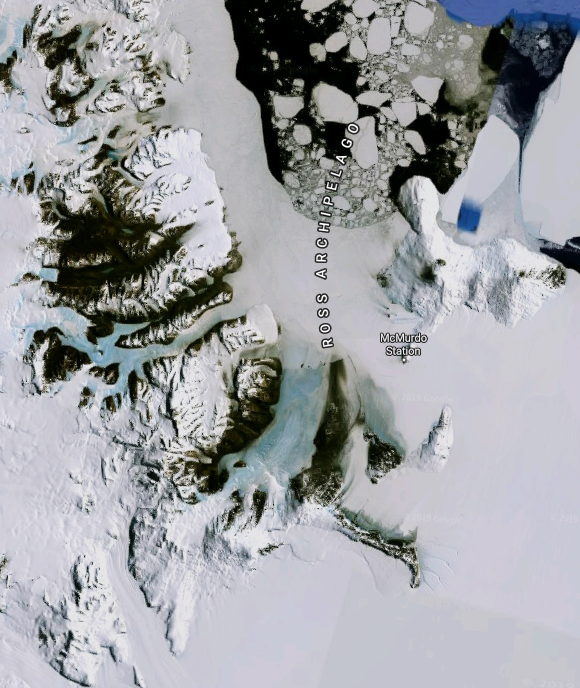
\includegraphics[width=0.5\textwidth]{dryvalleymap.png}
\caption{\label{fig:map} The general area of the dry valleys near Ross Island.}
\end{figure}
\end{frame}

\begin{frame}{What are the Dry Valleys?}
\begin{figure}
\centering
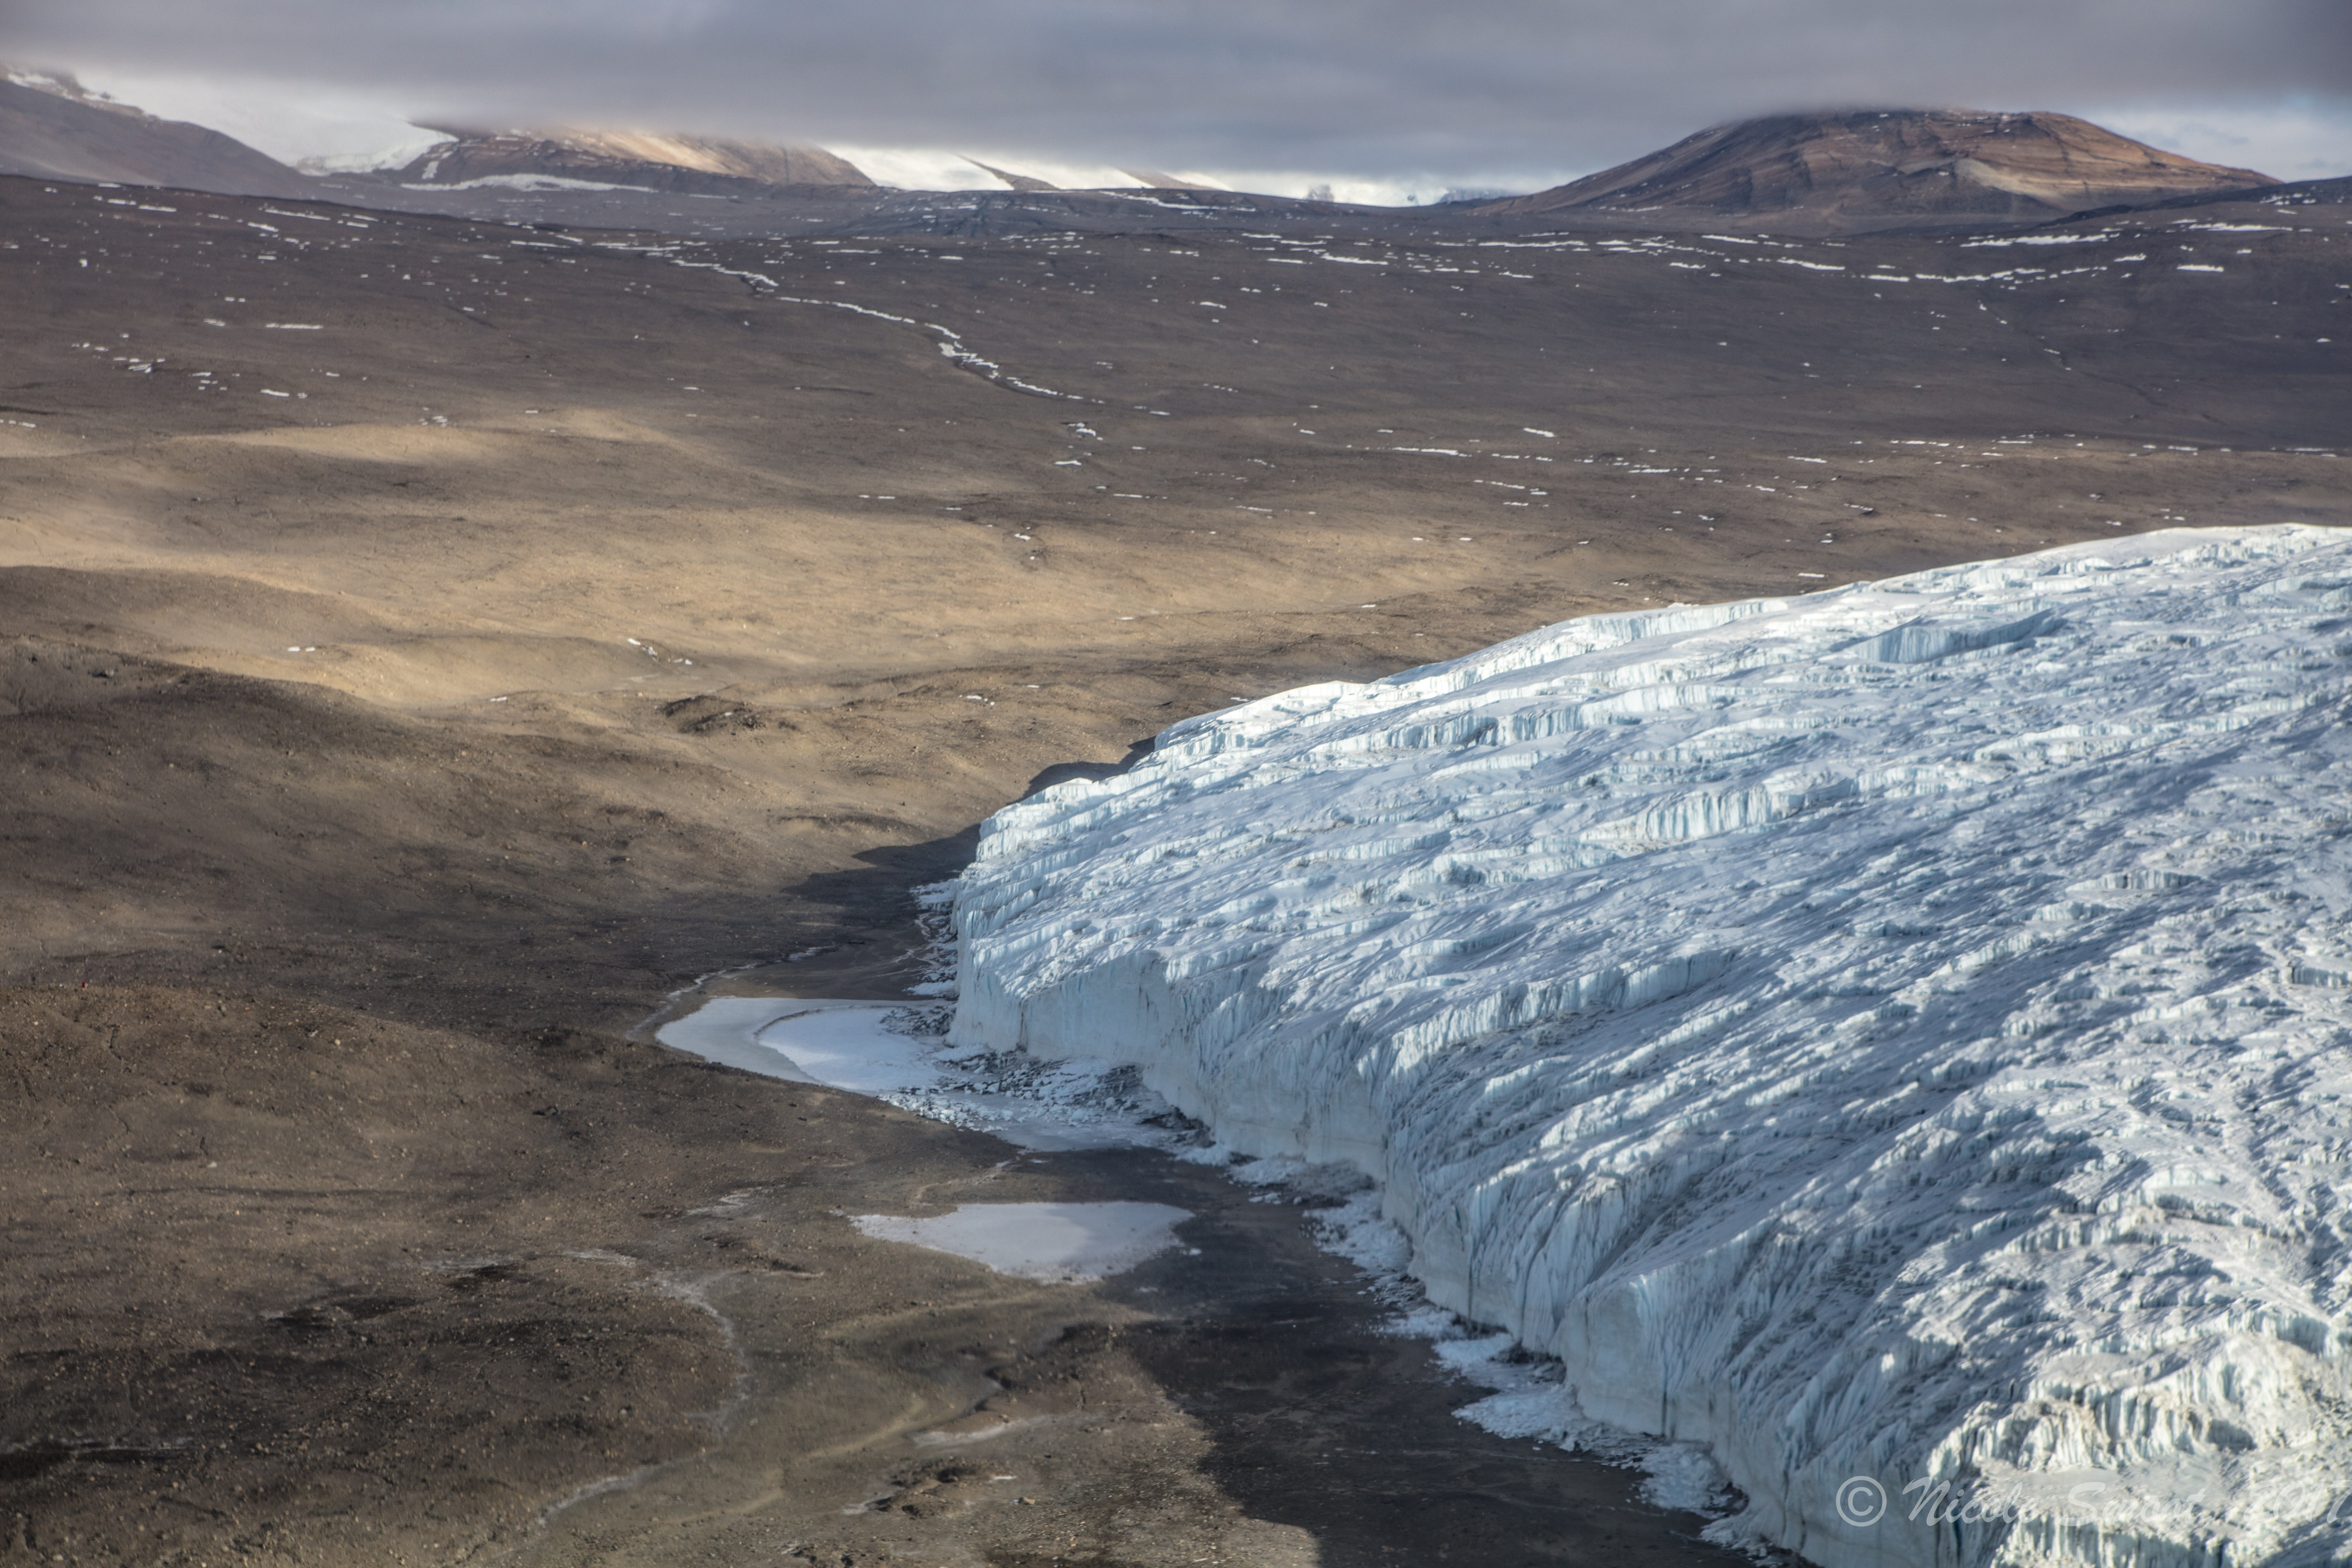
\includegraphics[width=0.75\textwidth]{dry1.jpg}
\caption{\label{fig:map1} A glacier in one of the three major valleys.}
\end{figure}
\end{frame}

\begin{frame}{What are the Dry Valleys?}
\begin{figure}
\centering
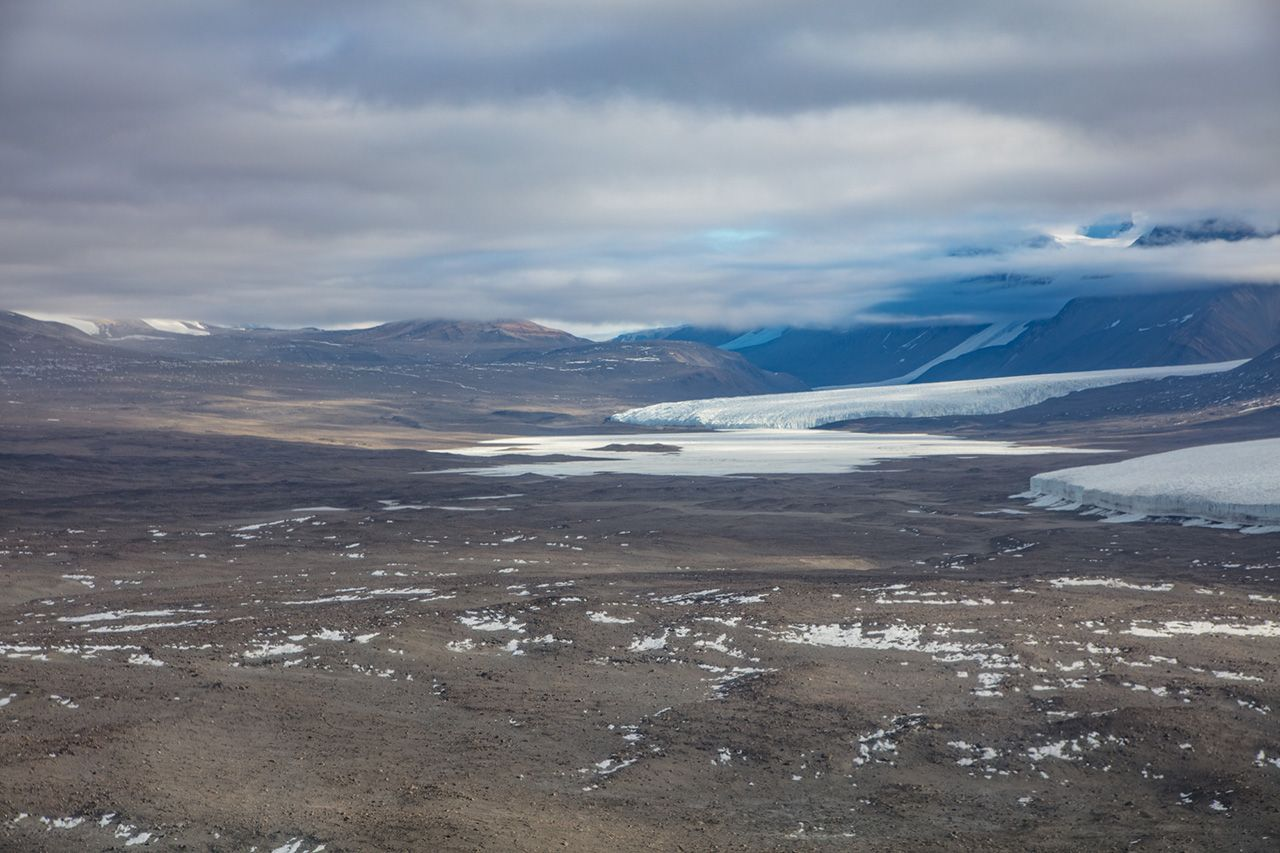
\includegraphics[width=0.75\textwidth]{dry2.jpg}
\caption{\label{fig:map2} A flat plain in one of the three major dry valleys.  One of the only places on Earth that has dry permafrost.}
\end{figure}
\end{frame}

\begin{frame}{What are the Dry Valleys?}
\begin{figure}
\centering
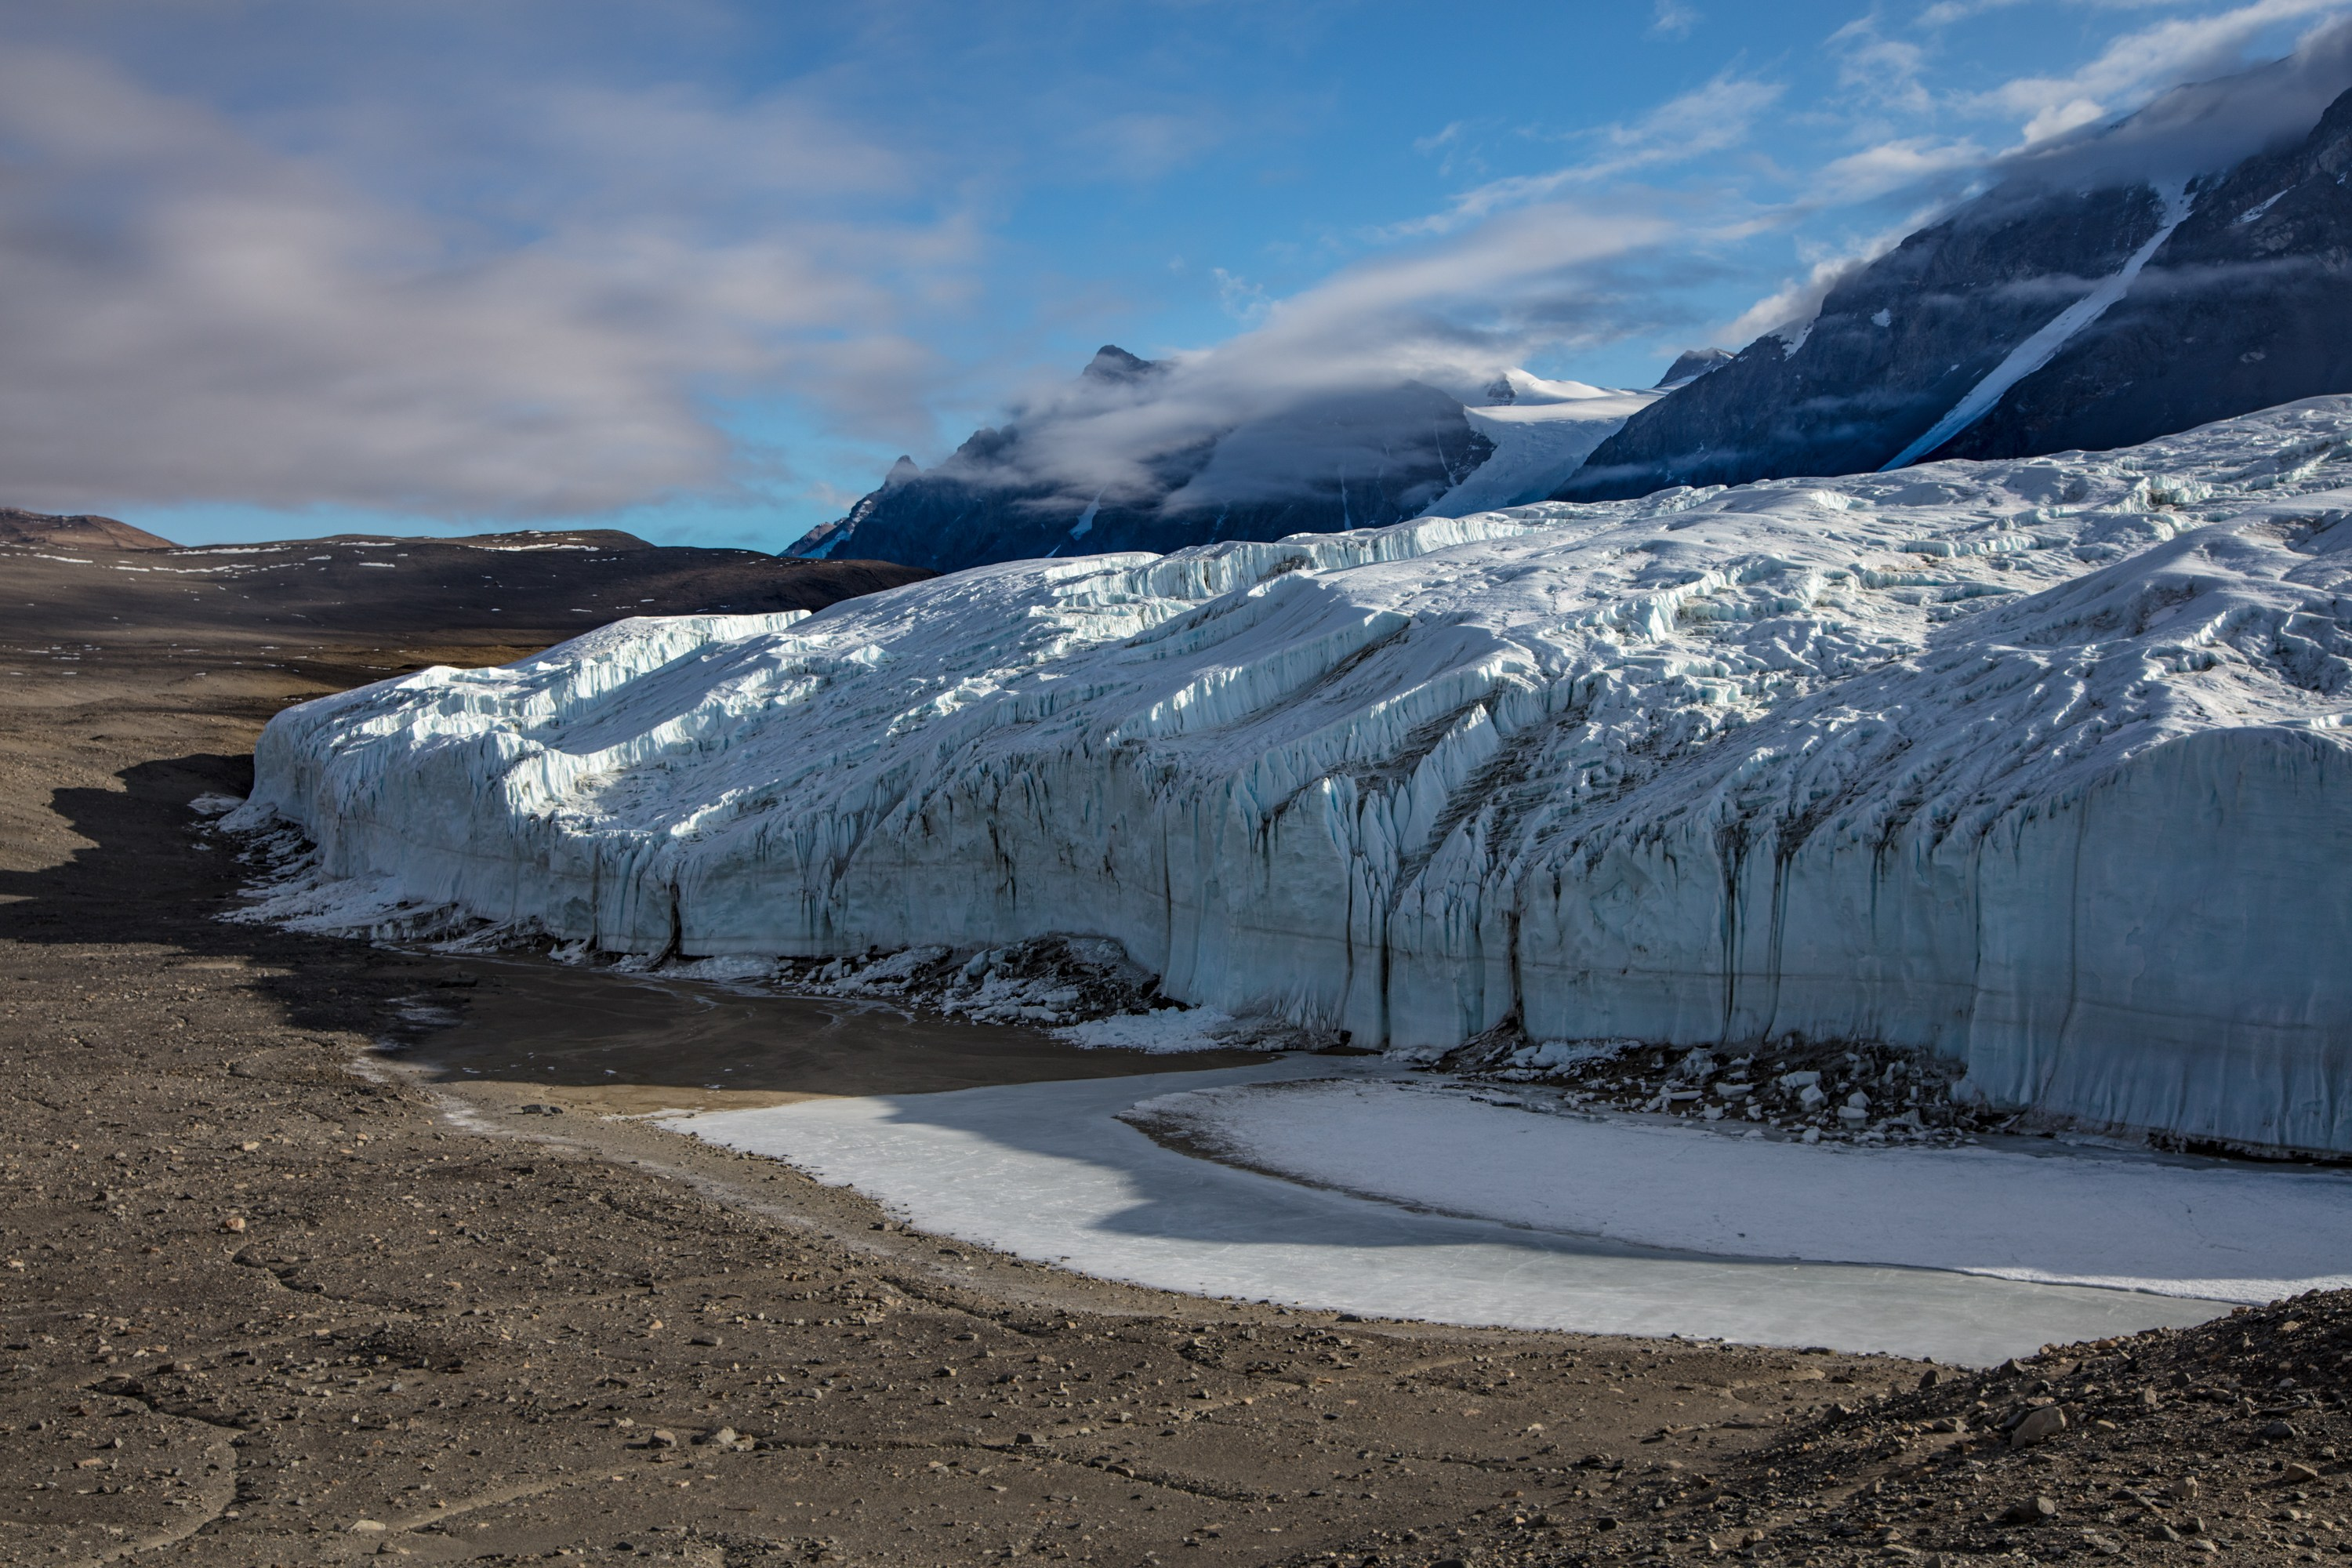
\includegraphics[width=0.75\textwidth]{dry3.jpg}
\caption{\label{fig:map3} There is almost no liquid water in the dry valleys due to katabatic winds and sublimation.}
\end{figure}
\end{frame}

\begin{frame}{What are the Dry Valleys?}
\begin{figure}
\centering
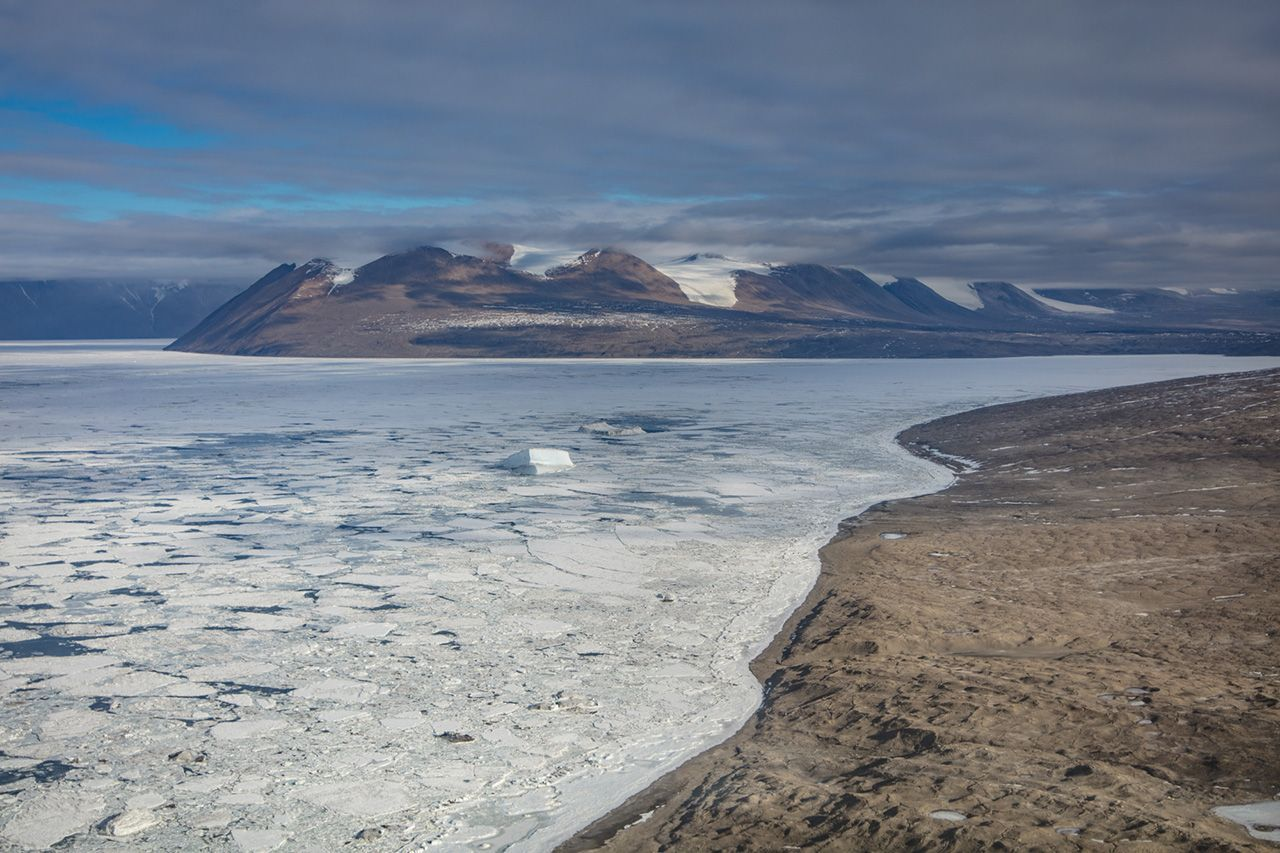
\includegraphics[width=0.75\textwidth]{dry4.jpg}
\caption{\label{fig:map4} The intersection of the dry valley areas and frozen ocean.  There is virtually no life in the entire area.}
\end{figure}
\end{frame}

\begin{frame}{What are the Dry Valleys?}
\begin{figure}
\centering
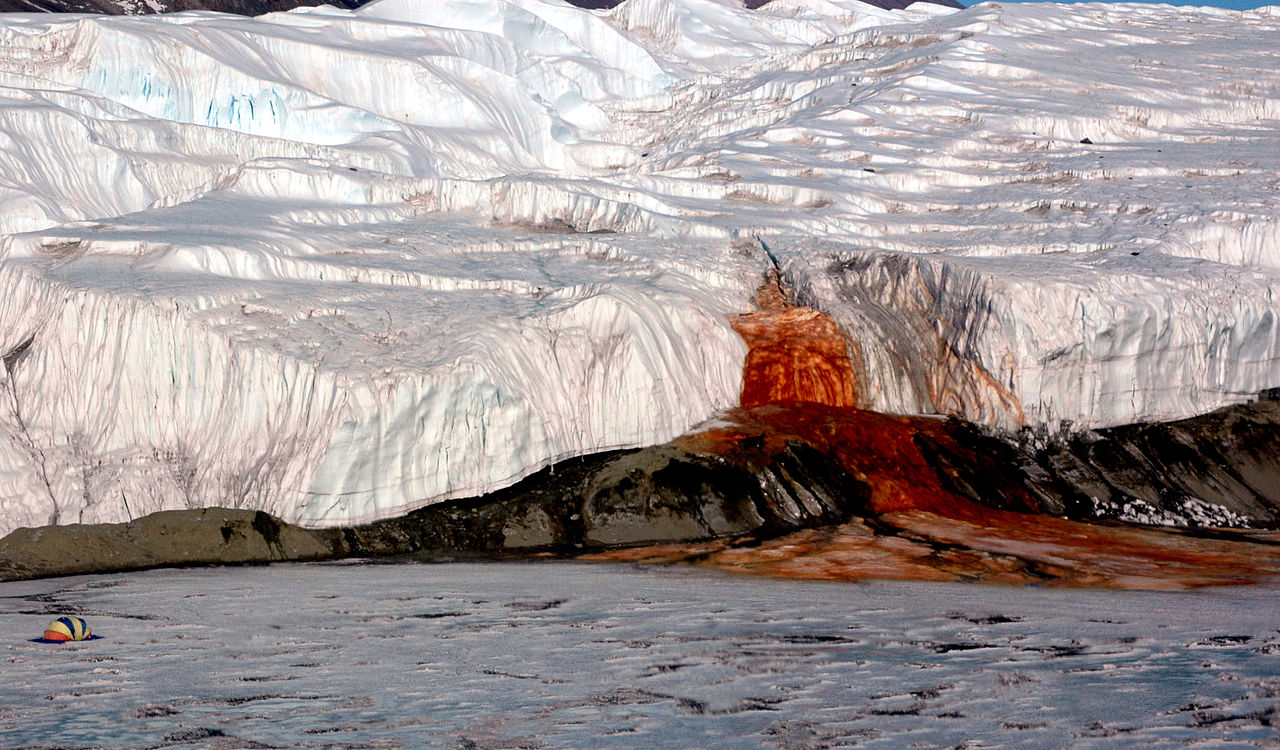
\includegraphics[width=0.75\textwidth]{blood.jpg}
\caption{\label{fig:blood} There is virtually no life in the entire area, but the soil has high concentrations of iron and other minerals.}
\end{figure}
\end{frame}

\begin{frame}{What are the Dry Valleys?}
\small
The three major valleys:
\begin{itemize}
\item \textbf{Taylor Valley:} The furthest south of the three valleys and home-sweet-home to Taylor Glacier and the infamous “Blood Waterfall”. Iron-oxide is what’s actually spewing out of the side of Taylor Glacier, although its resemblance to blood.
\item \textbf{Wright Valley:} The middle of the three valleys and home to the Onyx River, the largest river in all of Antarctica.
\item \textbf{Victoria Valley:} The northernmost valley of the McMurdo Dry Valleys and the location of Lake Vida, the largest lake of the three valleys.
\end{itemize}
\end{frame}

\begin{frame}{What are the Dry Valleys?}
Other facts about the Dry Valleys:
\begin{itemize}
\item Seen by Scott group in 1903 - concluded no life.
\item Katabatic winds, large swings in temperature (-2 deg C to 20 deg C surface temperature).
\item Researchers have found Endolithic photosynthetic bacteria within rocks found in the McMurdo Dry Valleys. These anaerobic bacteria survive by metabolizing sulfur and iron found beneath Taylor Glacier inside Taylor Dry Valley. 
\item These findings are what give the glimmer of the possibility of life on Mars.
\end{itemize}
\end{frame}

\begin{frame}{What are the Dry Valleys?}
\begin{figure}
\centering
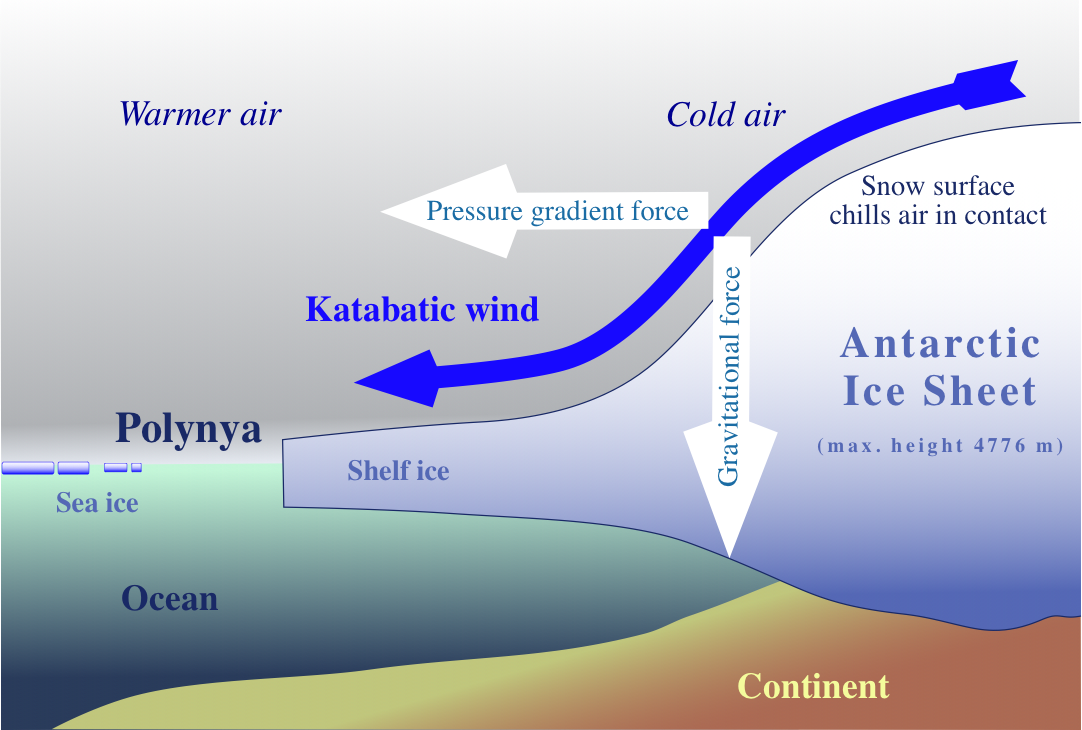
\includegraphics[width=0.6\textwidth]{kat.png}
\caption{\label{fig:kat} Simple diagram of katabatic wind.}
\end{figure}
\small
Two reasons that the dry valleys are dry:
\begin{itemize}
\item Katabatic winds
\item Trans-antarctic mountains act as precipitation barrier
\end{itemize}
\end{frame}

\section{The discovery of a bio-diverse bacterial profile in the Dry Valleys}

\begin{frame}
The basics of the discovery of bacterial diversity in the Dry Valleys:
\url{https://youtu.be/TAs-T3c-5ps}
\end{frame}

\section{Mars}

\begin{frame}{What are the Dry Valleys?}
\begin{figure}
\centering
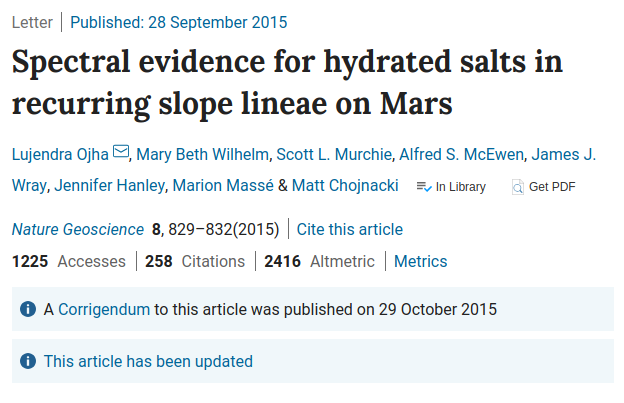
\includegraphics[width=0.6\textwidth]{paper.png}
\caption{\label{fig:mars} Discovery of brines flowing on Mars, in area of similar properties to the Dry Valleys.  (Exceptions: low pressure, larger temperature swings).}
\end{figure}
\end{frame}

\end{document}